\documentclass[a4paper, twoside, 12pt, listof=nochaptergap] {book}

%-----------------------------------------------
% packages.tex
% Package loading must be set here to ensure
% document's order
%-----------------------------------------------

% Typesetting and hyphenation helper %
\usepackage[indonesian]{babel}

% Text coloring %
\usepackage{color}

% Math typeset and equations and courier %
\usepackage{amsmath,amssymb,amsthm,mathtools}
\usepackage{courier}

% Every first paragraph is indented %
\usepackage{indentfirst}

% Paragraph spacing
\usepackage{setspace}

% For enumeration and the sorts %
\usepackage{enumitem}

% For styling titles and the sorts %
\usepackage{titlesec,titletoc}

% Table of Content needs %
\usepackage[titles]{tocloft}
\usepackage{tocbibind}

% For various "if" definitions %
\usepackage{etoolbox}

% Bibliography needs %
\usepackage[backend=bibtex,style=ieee,sorting=none]{biblatex}
\usepackage{url}

% Page margin %
\usepackage[top=4cm, bottom=4cm, left=3cm, right=3cm]{geometry}

% Paragraph alignment %
\usepackage{ragged2e}

% References debugging purpose: change 'final' to 'draft' to use %
\usepackage[final] {showkeys}

% Include pictures %
\usepackage{graphicx}
\usepackage{wrapfig}

% Code formatting %
\usepackage{listings}

% Captions formatting %
\usepackage{caption}
\usepackage{chngcntr}

% For tables need %
\usepackage{tabularx}

% Background %
\usepackage{eso-pic}

% Fonts -- compile with xelatex for correct output %
\usepackage{fontspec}

% Header-footer needs %
\usepackage{fancyhdr}

% Tables need to be rotated smh %
\usepackage{lscape}

% Drawing? %
\usepackage{tikz}
\usetikzlibrary{backgrounds}
\usetikzlibrary{shapes.geometric, arrows}

% Cool & fancy verbatim %
\usepackage{fancyvrb}

% Algorithm %
\usepackage[linesnumbered,boxed]{algorithm2e}

%-------------------------------------------------------------
% utils.tex
% Generic commands which may be used throughout the document
% should be set here
%-------------------------------------------------------------

%--
%  A set of command for appendix testing tables
%--
\newcommand {\testtableheader}
{
  \hline
  No & \multicolumn{3}{|c|}{BSGS}           & \multicolumn{3}{c|}{Brent} \\
  & \multicolumn{1}{|l}{R} & S & Verdict & R & S & Verdict        \\
  \hline
}

\newcommand {\testtablefooter}
{
  \hline
}

\newenvironment{testtable}
{
  \begin{tabular}{|l|l l l|l l l|}
  \testtableheader
}
{
  \testtablefooter
  \end{tabular}
}

%--
%  Shortcut command for QED symbol. Use it while in math environment
%--
\newcommand{\eop}{\ensuremath{\blacksquare}}

% Bugs in LaTeX are damn AMAZING %
%--
%  Preventing \addvspace to throw error due to unended paragraph
%  #1: Usual parameter entered
%--
\let\oldaddvspace\addvspace
\renewcommand\addvspace[1]
{
  \par\oldaddvspace{#1}
}

%--
%  Preventing \contentsline to throw error due to unended paragraph
%  #1, #2, #3: Usual parameter entered
%--
\let\oldcontentsline\contentsline
\renewcommand\contentsline[3]
{
  \par\oldcontentsline{#1}{#2}{#3}
}

%--
%  Creates a text to denote an empty page
%--
\newcommand\emptypage
{
  \begin{center}
    [\textit{Halaman ini sengaja dikosongkan}]
  \end{center}
  \newpage
}

%--
%  Works as if applying two \clearpage, plus some text denoting
%  the page is empty
%--
\makeatletter
\def\cleardoublepage
{
  \clearpage
  \if@twoside
    \ifodd\c@page
      % do nothing
    \else
      \emptypage
    \fi
  \fi
}
\makeatother
%---------------------------------------------------------%
%--          Labelling Utilities          --%
%---------------------------------------------------------%

%----------- 1 Document hierarchies

%--
%  Auto label chapter with proper prefix
%  Param
%  #1: Label name. If not given, #2 will be used
%  #2:  The shown name
%--
\makeatletter

\let\oldchapter\chapter

\newcommand{\chapterstar}[1]
{
  \oldchapter*{#1}
  \protect\label{sec:#1}
}

\newcommand{\chapternostar}[2][]
{
  \ifstrempty{#1}
    {\oldchapter{#2}\protect\label{sec:#2}}
    {\oldchapter[#1]{#2}\protect\label{sec:#1}}
}
\renewcommand{\chapter}{\@ifstar{\chapterstar}{\chapternostar}}

\makeatother

%--
%  Auto label section with proper prefix
%  Param
%  #1: Label name. If not given, #2 will be used
%  #2:  The shown name
%--
\let\oldsection\section
\renewcommand\section[2][]
{
  \protect\oldsection{#2}
  \ifstrempty{#1}{\protect\label{sec:#2}}{\protect\label{sec:#1}}
}

%--
%  Auto label subsection with proper prefix
%  Param
%  #1: Label name. If not given, #2 will be used
%  #2:  The shown name
%--
\let\oldsubsection\subsection
\renewcommand\subsection[2][]
{
  \protect\oldsubsection{#2}
  \ifstrempty{#1}{\protect\label{sec:#2}}{\protect\label{sec:#1}}
}

%--
%  Auto label subsubsection with proper prefix
%  Param
%  #1: Label name. If not given, #2 will be used
%  #2:  The shown name
%--
\let\oldsubsubsection\subsubsection
\renewcommand\subsubsection[2][]
{
  \protect\oldsubsubsection{#2}
  \ifstrempty{#1}{\protect\label{sec:#2}}{\protect\label{sec:#1}}
}

%--
%  Auto label paragraph with proper prefix
%  Param
%  #1: Label name. If not given, #2 will be used
%  #2:  The shown name
%--
\let\oldparagraph\paragraph
\renewcommand\paragraph[2][]
{
  \protect\oldparagraph{#2}
  \ifstrempty{#1}{\protect\label{sec:#2}}{\protect\label{sec:#1}}
}

%----------- 2 Environment

%--
%  Environment for code listings. Used for proper labelling
%  Param
%  #1: Additional key-value pair
%  #2:  Caption name
%  #3: Label name, automatically prefixed
%--
\lstnewenvironment{code}[3][]
{
  \lstset{
    caption=#2,
    label=code:#3,
    #1
  }
}{}
%----------------------------------------------------
% styles.tex
% Things which alter how the document would look
% but not necessarily to be implemented is to be set here
%----------------------------------------------------

%--    Listing    --%
\lstdefinestyle{generic}
{
  basicstyle=\ttfamily\footnotesize,
  tabsize=2,
  numbers=left,
  numbersep=0.6em,      % distance between number and code
  numberstyle=\footnotesize\ttfamily\itshape,
  numberfirstline=false,
  xleftmargin=2.2em,    % starting margin exclusively for the code
  frame=single,      % frame type
  framexleftmargin=2.3em,  % distance between left frame to the element in the listing}
  framerule=1pt,
  breaklines=true,
  breakatwhitespace=true,
  breakindent=20pt,
  captionpos=b,
  escapechar=~
}

%--    Header-footer    --%
\fancypagestyle{normal}
{
  \fancyhf{}  % Remove all setting
  \fancyhead[LE,RO] {\thepage}
  \renewcommand {\headrulewidth}{0pt}
  \renewcommand {\footrulewidth}{0pt}
}
%------------------------------------------
% variables.tex
% All key-value pair should be set here
%------------------------------------------

% Variables declaration %
\def \judul {Pengembangan Algoritma Pencarian Non Interaktif untuk Penyelesaian Permasalahan Pencarian Ulam dengan Kebohongan Jamak}
\def \penulis {Risyanggi Azmi Faizin}
\def \oj {Sphere Online Judge}
\def \soal {Guess The Number v5}
\def \nomorsoal {1598}
\def \nrplama {5116201052}
\def \nrpbaru {05111650010052}
\def \jurusanlama {Jurusan Teknik Informatika}
\def \jurusanbaru {Departemen Informatika}
\def \fakultaslama {Fakultas Teknologi Informasi}
\def \fakultasbaru {Fakultas Teknologi Informasi dan Komunikasi}
\def \pembimbingsatu {Dr. Ir. R. V. Hari Ginardi, M.Sc}
\def \nikpembimbingsatu {196505181992031003}

\def \juduleng {Development of Non-Interactive Searching Algorithm for Solving Ulam's Searching Problem with Many Lies}
\def \jurusanlamaeng {Informatics Department}
\def \jurusanbarueng {Informatics Department}
\def \fakultaslamaeng {Faculty of Information Technology}
\def \fakultasbarueng {Faculty of Information and Communication Technology}

\definecolor{abucover}{RGB}{128,128,128}
%---------------------------------------------------------
% setting.tex
% Everything that covers about the document setting
% and must be in preamble is to be implemented right here
%---------------------------------------------------------

%--    Whole document paragraph    --%
\setlength{\parindent}{2.5em}
\setlength{\parskip} {0.2em}
\setstretch{1.5}

\setlist[enumerate] {itemsep=0pt, topsep=6pt, partopsep=0pt, parsep=0pt}

%--    Redactions    --%
\captionsetup[table] {skip=-6pt, name={Tabel }}
\captionsetup[figure] {skip=6pt,name={Gambar }}
\captionsetup[algorithm] {skip=6pt,name={Algoritma }}

\AtBeginEnvironment{algorithm}{\setstretch{1}}

% Babel is weird
\addto\captionsindonesian
{
  \renewcommand{\lstlistingname}{Kode Sumber}
  \renewcommand{\chaptername}{BAB}
  \renewcommand{\contentsname}{DAFTAR ISI}
  \renewcommand{\listfigurename}{DAFTAR GAMBAR}
  \renewcommand{\listtablename}{DAFTAR TABEL}
  \renewcommand{\lstlistlistingname}{DAFTAR KODE SUMBER}
}

%--    Document hierarchy depth    --%
\setcounter{secnumdepth}{5}

%--    Document fonts    --%
\setmainfont{Times New Roman}
\setmonofont{Courier New}

%--    Set the \chapter    --%
\titleformat{\chapter}        % section
[display]              % shape
{\Centering\bfseries}        % format
{\chaptername \ \Roman{chapter}}  % label
{0.4ex}                % label-section separator
{}                  % before code
[]                  % after

% for unknown reason, spacing should be set using the following format
\titlespacing*{\chapter}{0pt}{-20pt}{20pt}

%--    Set the \chapter*    --%
\titleformat{name=\chapter,numberless}  % section
[display]          % shape
{\Centering\bfseries}    % format
{}              % label
{0.4ex}            % label-section separator
{}              % before code
[]              % after

%--    Set the \section    --%
\titleformat{\section}
[hang]
{\bfseries}
{\thesection. }
{0ex}
{}
[\vspace{-0.9em}]

%--    Set the \subsection    --%
\titleformat{\subsection}
[hang]
{\bfseries}
{\thesubsection. }
{0ex}
{}
[\vspace{-0.6em}]

%--    Set the \subsubsection    --%
\titleformat{\subsubsection}
[hang]
{\bfseries}
{\thesubsubsection. }
{0ex}
{}
[\vspace{-0.6em}]

%--    Listing    --%
\lstset{style=generic}
\makeatletter
\def\lst@PlaceNumber{\ifnum\value{lstnumber}=0\else
  \llap{\normalfont\lst@numberstyle{\thelstnumber}\kern\lst@numbersep}\fi}
\makeatother

%--    Bibliography    --%
\defbibheading {bibliography}[DAFTAR PUSTAKA]{\chapter{#1}}
\urlstyle{rm}

%--    Table of Content  --%
\setlength\cftparskip{-2pt}
\setlength\cftbeforechapskip{0pt}
\setlength{\lineskip}{0pt}

% Chapter uses roman numeral
\renewcommand{\cftchapleader}{\cftdotfill{\cftdotsep}}
\newcommand{\Romannumeral}[1]{\uppercase\expandafter{\romannumeral#1}}
\renewcommand{\cftchappresnum}{\chaptername \ \Romannumeral}

% Prefix each segment
\renewcommand{\cfttabpresnum}{Tabel }
\renewcommand{\cftfigpresnum}{Gambar }

% Set each segment's indentation such that none will overlap
\cftsetindents{chapter}{0em}{4.4em}
\cftsetindents{section}{2em}{2em}
\cftsetindents{figure}{0em}{6em}
\cftsetindents{table}{0em}{5em}

% Theorems
\newtheorem{theorem}{Theorem}[section]
\newtheorem{corollary}{Corollary}[theorem]
\newtheorem{exmp}{Example}[section]
\newtheorem{lemma}[theorem]{Lemma}

% Algorithm
\renewcommand{\algorithmcfname}{Kode sumber}
\renewcommand{\algorithmautorefname}{kode sumber}
\renewcommand{\listalgorithmcfname}{Daftar kode sumber}
\SetAlCapSty{}
\SetKwProg{Fn}{Function}{}{end}
\SetAlCapSkip{1em} %ini antara caption sama body, padahal mksdku itu caption sama paragraphnya
\DontPrintSemicolon

%---------------------------------------------------------
%  List of how words in Indonesian should be hyphenated
%---------------------------------------------------------

% Mathematic specific
\hyphenation{kong-ru-en-si}
\hyphenation{mo-du-lo}
\hyphenation{mo-du-lus}
\hyphenation{mul-ti-pli-ca-tive}
\hyphenation{or-der}
\hyphenation{lo-ga-rit-ma dis-kret}
\hyphenation{ex-po-nent}
\hyphenation{in-vers}
\hyphenation{te-o-re-ma}
\hyphenation{lo-ga-rit-mik}
\hyphenation{lo-ga-rith-mic}
\hyphenation{pro-por-si}
\hyphenation{fak-to-ri-sa-si}
\hyphenation{kar-di-na-li-tas}
\hyphenation{po-li-no-mi-al}
\hyphenation{po-ly-no-mi-al}  
\hyphenation{stan-dar de-vi-a-si}

\hyphenation{pol-lard rho}
\hyphenation{ba-by step gi-ant step}
\hyphenation{euler to-tient func-ti-on}

% Problem specific
\hyphenation {dsa at-tack}
\hyphenation {sig-na-tu-re}
\hyphenation {run-ti-me}
\hyphenation {krip-to-gra-fi}
\hyphenation {re-pe-at-ed squ-a-ring}
\hyphenation {ge-ne-ra-tor}
\hyphenation {pu-blic}
\hyphenation {pri-va-te}
\hyphenation {key}
\hyphenation {pri-mi-ti-ve root}
\hyphenation {bru-te for-ce}
\hyphenation {ran-dom func-ti-on}
\hyphenation {step}
\hyphenation {in-te-ger o-ver-flow}
\hyphenation {mul-ti-pli-ca-ti-on}
\hyphenation {ex-po-nent-i-a-ti-on}
\hyphenation {pri-ma-li-ty}
\hyphenation {strong li-ar}
\hyphenation {pro-ba-bi-lis-tik}
\hyphenation {de-ter-mi-nis-tik}
\hyphenation {struct}
\hyphenation {po-int-er}

% Miscellaneous
\hyphenation {meng-ha-sil-kan}
\hyphenation {a-kan}
\hyphenation {ber-ja-lan}
\addbibresource{holy.bib}

\begin{document}
  %-- Things that should go first but can't be placed in preamble
  % Figure numbering uses chapter numbering as prefix
  \counterwithin {figure}{chapter}

  \pagestyle {normal}
  %--

  \frontmatter
    \newpage
  \newgeometry{top=9cm,left=3cm,bottom=2cm}

  \sffamily
  \thispagestyle{empty}
  \begin{spacing}{2.0}
    {\noindent
      \textbf{BUKU TESIS - KI2501}\\*[20pt]
      {\large\textbf{\MakeUppercase{\judul}}} \\*[20pt]
    }
  \end{spacing}
  \begin{spacing}{1.3}
  {\large \noindent
    \MakeUppercase{\penulis} \\*
    NRP \nrplama \\*[20pt]
    Dosen Pembimbing\\*
    \pembimbingsatu \\
    NIP: \nikpembimbingsatu \\*[20pt]
    Program Magister\\
    Rumpun Mata Kuliah Algoritma dan Pemrograman\\
    \MakeUppercase{\jurusanbaru} \\*
    \fakultasbaru \\*
    Institut Teknologi Sepuluh Nopember \\*
    Surabaya, 2018
  }
  \end{spacing}
  \AddToShipoutPictureBG*{
\includegraphics[width=\paperwidth,height=\paperheight]{../img/cover1.png}}
  \rmfamily
  \normalsize
  \restoregeometry
  \cleardoublepage

\newpage
  \newgeometry{top=9cm,left=3cm,bottom=2cm}

  \sffamily
  \thispagestyle{empty}
  \begin{spacing}{2.0}
    {\noindent
      \textbf{BUKU TESIS - KI2501}\\*[20pt]
      {\large\textbf{\MakeUppercase{\judul}}} \\*[20pt]
    }
  \end{spacing}
  \begin{spacing}{1.3}
  {\large \noindent
    \MakeUppercase{\penulis} \\*
    NRP \nrplama \\*[20pt]
    Dosen Pembimbing\\*
    \pembimbingsatu \\
    NIP: \nikpembimbingsatu \\*[20pt]
    Program Magister\\
    Rumpun Mata Kuliah Algoritma dan Pemrograman\\
    \MakeUppercase{\jurusanbaru} \\*
    \fakultasbaru \\*
    Institut Teknologi Sepuluh Nopember \\*
    Surabaya, 2018
  }
  \end{spacing}
  \AddToShipoutPictureBG*{
\includegraphics[width=\paperwidth,height=\paperheight]{../img/cover2.png}}
  \rmfamily
  \normalsize
  \restoregeometry
  \cleardoublepage
  
\newpage
  \newgeometry{top=9cm,left=3cm,bottom=2cm}

  \sffamily
  \thispagestyle{empty}
  \begin{spacing}{2.0}
    {\noindent
      \textbf{BUKU TESIS - KI2501}\\*[20pt]
      {\large\textbf{\MakeUppercase{\juduleng}}} \\*[20pt]
    }
  \end{spacing}
  \begin{spacing}{1.3}
  {\large \noindent
    \MakeUppercase{\penulis} \\*
    NRP \nrplama \\*[20pt]
    Supervisor\\*
    \pembimbingsatu \\
    NIP: \nikpembimbingsatu \\*[20pt]
    Program Magister\\
    Algorithms and Programming\\
    \MakeUppercase{\jurusanbarueng} \\*
    \fakultasbarueng \\*
    Institut Teknologi Sepuluh Nopember \\*
    Surabaya, 2018
  }
  \end{spacing}
  \AddToShipoutPictureBG*{
\includegraphics[width=\paperwidth,height=\paperheight]{../img/cover2.png}}
  \rmfamily
  \normalsize
  \restoregeometry
  \cleardoublepage
    % \include {buku/lembar_pengesahan}
    % ---- Indonesian vers.
\chapter {ABSTRAK}
\noindent\textbf{\MakeUppercase\judul}
\vspace*{1em}

\begin{tabularx}{\linewidth}{ l l X }
  Nama       & : & \penulis \\
  NRP       & :  & \nrplama \\
  % Departemen     & : & \jurusanbaru, \newline \fakultasbaru, ITS \\
  Pembimbing     & : & \pembimbingsatu
  \vspace*{1em}   % HACKY--USE ALTERNATIVE IF POSSIBLE %
\end{tabularx}

\noindent\textbf{\large Abstrak} \\
\itshape
Pada permasalahan permainan klasik pencarian Ulam dan Rényi, penanya harus mengajukan beberapa pertanyaan iya dan tidak untuk mencari sebuah nilai dalam range pencarian yang sudah disepakati, namun penjawab diperbolehkan berbohong. Sudah ada solusi dari beberapa variasi pada permasalahan pencarian Ulam dan Rényi, yaitu pada jenis query antara rentang atau subset dan jumlah maksimal bohong antara satu, dua, tiga, dan seterusnya. Namun belum ada solusi yang sempurna untuk query yang non interaktif yaitu penjawab hanya boleh menjawab query penanya setelah penanya selesai menanyakan semua querynya. Belum ada penelitian yang menyelesaikan permasalahan ini. Pada paper ini akan dijelaskan solusi sempurna untuk permainan Ulam dan Rényi non interaktif dengan maksimal kebohongan jamak menggunakan kode biner dengan jarak Hamming. Hasil algoritma pada paper ini menunjukkan jumlah query yang jauh lebih sedikit dari algoritma umum repetisi biner dan hasil terbaik pada pengujian online ternama.

\vspace*{1em}
\noindent\bfseries Kata Kunci: permainan ulam; bohong; jarak hamming; kode biner; query;
\normalfont
\cleardoublepage

% ---- English vers.
\chapter {ABSTRACT}
\noindent\textbf{\MakeUppercase\juduleng}
\vspace*{1em}

\begin{tabularx}{\linewidth}{ l l X }
  Name       & : & \penulis \\
  Student ID    & :  & \nrplama \\
  % Department     & : & \jurusanbarueng, \newline \fakultasbarueng, ITS \\
  Supervisor    & : & \pembimbingsatu
  \vspace*{1em}   % HACKY--USE ALTERNATIVE IF POSSIBLE %
\end {tabularx}

\noindent\textbf{\large Abstract} \\
\itshape
On the classic Ulam and Rényi searching problem, the questioner has to ask some yes-no questions to find an unknown value within the agreed search space, but the answerer is allowed to lie. There are already solutions of some variations in the Ulam and Rényi searching problem, i.e. on the type of query between range or subset and the maximum number of lies between one, two, three, and so on. But there is no perfect solution for non-interactive queries which the answerer can only answer the questioner's query after the questioner has finished querying all the queries. No research has resolved this problem yet. In this paper we will describe the perfect solution for non-interactive Ulam and Rényi searching problem with many lies using binary code with Hamming distance. The algorithm results in this paper shows a much smaller number of queries than the common binary repetition algorithm and the best results on a reputable online judge.

\vspace*{1em}
\noindent\bfseries Keywords: ulam game; lies; hamming distances; binary codes; query;
\normalfont
\cleardoublepage
    \chapter {KATA PENGANTAR}

Bismillahirrohmaanirrohiim. Puji syukur penulis panjatkan kepada Tuhan Yang Maha Esa. Atas rahmat dan kasih sayangNya, penulis dapat menyelesaikan tesis dalam bentuk buku ini yang berjudul \textbf{\judul}.

Pengerjaan buku ini penulis tujukan untuk mengeksplorasi lebih mendalam topik-topik yang tidak diwadahi oleh kampus, namun banyak menarik perhatian penulis. Selain itu besar harapan penulis bahwa pengerjaan tugas akhir sekaligus pengerjaan buku ini dapat menjadi batu loncatan penulis dalam menimba ilmu yang bermanfaat.

Penulis ingin menyampaikan rasa terima kasih kepada banyak pihak yang telah membimbing, menemani dan membantu penulis selama masa pengerjaan tesis maupun masa studi.

\begin {enumerate}
  \item Allah SWT yang selalu memberi kebahagiaan dan makna pada hidup.
  \item Ibu dan Ayah yang selalu mendukung dalam segala-gala-gala hal. Terbaik.
  \item Bapak Rully Soelaiman S.Kom.,M.Kom., selaku pembimbing bayangan penulis. Ucapan terima kasih juga penulis sampaikan atas segala perhatian, didikan, pengajaran, dan nasihat yang telah diberikan oleh beliau selama masa studi penulis.
  \item Bapak \pembimbingsatu, selaku pembimbing penulis yang telah memberikan arahan semasa pengerjaan tesis.
  \item Rekan-rekan satu angkatan 2016 mahasiswa magister Teknik Informatika yang tidak lelah membantu penulis semasa masa studi, juga karena kesabaran mereka yang luar biasa dalam menghadapi kelakuan penulis.
  \item Rekan-rekan satu lab DTK yang senantiasa memberi kebahagiaan nyata meskipun hanya sementara.
\end {enumerate}

Penulis menyadari bahwa buku ini jauh dari kata sempurna. Maka dari itu, penulis memohon maaf apabila terdapat salah kata maupun makna pada buku ini. Akhir kata, penulis mempersembahkan buku ini sebagai wujud nyata kontribusi penulis dalam ilmu pengetahuan.

\begin{flushright}
Surabaya, Juni 2018 \\*
\vspace{5em}
\penulis
\end{flushright}
    \tableofcontents\cleardoublepage
\listoffigures\cleardoublepage
\listoftables\cleardoublepage
% \lstlistoflistings\cleardoublepage
{\let\clearpage\relax\listofalgorithms}\cleardoublepage

  \mainmatter
    \vspace{0ex}
\chapter {PENDAHULUAN}
Pada bab ini, akan dijelaskan mengenai latar belakang, rumusan masalah, Batasan masalah, tujuan, metodologi pengerjaan, dan sistematika penulisan tesis.

\section{Latar Belakang}
\par Dalam perkembangan dunia teknologi informasi selama beberapa dekade terakhir, teknologi informasi seringkali dijadikan solusi bagi permasalahan-permasalahan yang pernah ada, yang sebelumnya diselesaikan secara manual oleh manusia. Contoh permasalahan yang pernah ada adalah salah satu permasalahan klasik pencarian Ulam dan Rényi. Permasalahan ini dapat diilustrasikan dengan adanya dua pemain yang disebut penanya dan penjawab. Diberikan range pertanyaan $S_M = {0,\ldots,M-1}$, penjawab menentukan sebuah bilangan $x \in S_M$. Penanya harus menemukan nilai $x$ dengan memberikan beberapa query berupa pertanyaan iya dan tidak, apakah "$x \in Q$?", di mana $Q$ adalah subset dari $S_M$, lalu penjawab menjawab "ya" atau "tidak". Permasalahan utama adalah penjawab dapat berbohong sampai $e$ kali. Masalah dari permainan ini adalah mencari jumlah query minimal untuk dapat menentukan nilai $x$.

Pada permasalahan pencarian Ulam, penanya dan penjawab harus menyepakati beberapa peraturan sebelum bermain. Peraturan tersebut meliputi batasan ruang pencarian, batasan bagaimana penjawab diperbolehkan berbohong, format pertanyaan, dan bagaimana interaksi antara penjawab dan penanya \cite{Pelc2002}. Pertama penanya dan penjawab harus menyepakati batas ruang pencarian $S_M$, yaitu $M$ angka, penjawab hanya boleh menentukan angka $x$ diantara dalam set $\{0,\ldots,M-1\}$.

Aturan bagaimana penjawab diperbolehkan berbohong adalah aturan yang fundamental dalam permainan pencarian Ulam dan Rényi. Aturan probabilitas berbohong dicetuskan oleh Rényi dan aturan jumlah bohong dicetuskan oleh Ulam \cite{StanislawMUlam1976}. Pada kebohongan probabilitas yang diikiat secara global, probabilitas penjawab melakukan kebohongan ditentukan oleh $r$, sehingga maksimal penjawab melakukan kebohongan adalah $rn$ di mana $n$ adalah jumlah pertanyaan dan $r<1$ \cite{Dhagat1999}. Pada aturan jumlah bohong, variasi beragam antara maksimal penjawab dapat berbohong hanya satu \cite{Ellis2008} \cite{Pelc1988}, dua \cite{Cicalese2000}, tiga \cite{Negro1992}, dan lebih dari tiga \cite{Berlekamp1998} \cite{Deppe2004}.

Pada aturan format pertanyaan, terdapat beberapa variasi. Yang pertama adalah pertanyaan komparasi, bentuk pertanyaannya adalah "Apakah $x<a$?" di mana $a \in S_M$ \cite{Innes} \cite{Auletta1992}. Lalu ada pertanyaan interval dan bi-interval, bentuk pertanyaannya adalah "Apakah $x$ ada dalam interval $[a,b]$?" \cite{Peter2017} dan "Apakah $x$ ada dalam interval $[a,b] \cup [c,d]$?" \cite{Mundici1997}. Lalu format pertanyaan subset, bentuk pertanyaannya adalah "Apakah $x$ ada dalam $A$ di mana $A \subseteq S_M$" \cite{Katona} \cite{Macula1997}.

Pada aturan interaksi antara penjawab dan penanya, terdapat tiga macam variasi yaitu interaktif, batch, dan non interaktif. Aturan yang paling umum digunakan adalah interaktif, yaitu penjawab harus menjawab setiap pertanyaan yang diajukan penanya sebelum penanya menanyakan pertanyaan selanjutnya. Pada aturan batch, penanya dan penjawab menyepakati berapa jumlah batch. Lalu pada setiap batch, penanya memberikan beberapa pertanyaan, lalu penjawab memberikan jawaban sejumlah pertanyaan yang diberikan oleh penanya \cite{Cicalese2000}. Aturan yang terakhir adalah non interaktif, yaitu penjawab harus menjawab semua pertanyaan penanya sekaligus \cite{Macula1997}.

Salah satu variasi permasalahan Ulam dan Rényi yang diangkat dalam penelitian ini adalah pencarian Ulam dengan $n$ query subset ${q_1,q_2,\ldots,q_n} | q_i \in S_M$, maksimal bohong adalah $e$, dan penjawab hanya boleh menjawab query penanya setelah penanya selesai menanyakan semua query-nya. Belum ada penelitian yang menyelesaikan permasalahan ini. Oleh karena itu penelitian ini bertujuan untuk memberikan solusi pada permasalahan ini.


\section {Rumusan Masalah}
Permasalahan yang akan diselesaikan pada tesis ini adalah sebagai berikut:

\begin {enumerate}
  \item Bagaimana merumuskan query untuk mencari bilangan diskrit pada interval yang diberikan pada permasalahan pencarian Ulam dengan pertanyaan seminimal mungkin?
  \item Apakah algoritma kode biner dengan jarak Hamming dapat menyelesaikan permasalahan pencarian Ulam non interaktif lebih baik?
  \item Bagaimana implementasi struktur data yang efisien dan optimal untuk menyelesaikan permasalahan pencarian Ulam?
  \item Apakah solusi meggunakan algoritma kode biner dengan tabel pencarian dapat diterima pada pengujian online SPOJ?
\end {enumerate}


\section {Batasan Masalah}
Masalah yang akan diselesaikan memiliki batasan-batasan berikut:

\begin {enumerate}
  \item Implementasi algoritma menggunakan bahasa pemrograman C++.
  \item Batas maksimum kasus uji adalah $2^7$.
  \item Interval bilangan yang yang dicari berada pada $[1,n]$, dengan $n$ maksimum $2^{12}$.
  \item Dataset yang digunakan adalah dataset pada permasalahan SPOJ GUESSN5.
\end {enumerate}


\section {Tujuan}
Tujuan tesis ini adalah sebagai berikut:

\begin{enumerate}
  \item Melakukan analisis dan mendesain algoritma dan struktur data untuk mencari bilangan dengan kebohongan dalam studi kasus permasalahan pencarian Ulam non interaktif dengan kebohongan.
  \item Mengevaluasi hasil dan kinerja algoritma dan struktur data yang telah dirancang untuk permasalahan pencarian Ulam non interaktif dengan kebohongan.
\end{enumerate}


\section {Sistematika Penulisan}
Sistematika laporan tesis yang akan digunakan adalah sebagai berikut:

\begin{enumerate}
\item Bagian awal, meliputi halaman depan, halaman pengesahan, abstrak, kata pengantar, daftar isi, daftar gambar, dan daftar tabel.
\item Bagian inti, meliputi pendahuluan, tinjauan pustaka, metodologi, hasil dan pembahasan, dan kesimpulan dan saran.
\item Bagian akhir, meliputi daftar pustaka, lampiran-lampiran, dan biodata penulis.
\end{enumerate} \cleardoublepage
    \chapter {DASAR TEORI}

Pada bab ini, dasar teori yang digunakan sebagai landasan pengerjaan tugas akhir ini akan dijabarkan.

\section{Problem formulation}

Bentuk permasalahan Ulam yang dibahas pada paper ini diangkat dari online judge SPOJ oleh Micha\l{} Miodek \cite{guessn5}. Penjawab menentukan sebuah bilangan $x$ pada rentang $S_M=\{0,\ldots,M-1\}$. Anda sebagai penanya harus mencari nilai $x$ dengan memberikan maksimal $n$ query khusus apakah "$x \in Q$?", lalu penjawab menjawab "ya" atau "tidak" pada setiap query yang ditanyakan. Permasalahan utama adalah penjawab dapat berbohong sampai $e$ kali. Selain itu, penjawab hanya boleh menjawab query penanya setelah penanya selesai menanyakan semua query-nya. Tujuan dari Ulam adalah mencari jumlah query minimal untuk dapat menentukan nilai $x$.

Bentuk dari query adalah string $s_1s_2s_3\ldots s_n$ dimana si bernilai '0' atau '1'. Jawaban dari penjawab adalah "Ya" jika $s_x=1$ atau "Tidak" jika $s_x=0$ dengan asumsi penjawab menjawab jujur.

Tugas sesungguhnya dari permasalahan ini adalah bukan untuk mencari nilai $x$, tapi hanya menyiapkan query yang dapat memeungkinkan untuk mendapatkan nilai $x$ dari semua kemungkinan jawaban dari penjawab. Penjawab tidak akan menjawab query yang diberikan penanya. Jika penjawab menemukan ada suatu set jawaban yang menyebabkan lebih dari satu kemungkinan nilai $x$, maka pengujian dianggap gagal.

Batasan yang digunakan pada permasalahan Ulam adalah sebagai berikut:
\begin{itemize}
  \item Batas maksimum kasus uji adalah $2^7$.
  \item Interval bilangan yang yang dicari berada pada $\{0,\ldots,M-1\}$, dengan n maksimum $2^{12}$.
  \item Dataset yang digunakan adalah dataset pada permasalahan SPOJ GUESSN5.
\end{itemize}

\begin{figure}
\centering
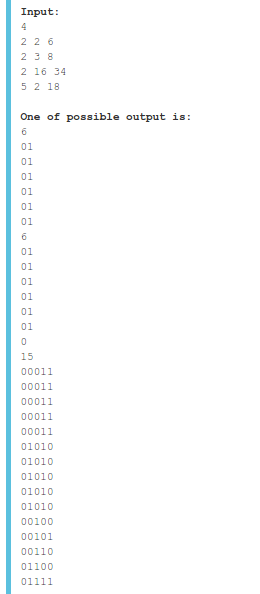
\includegraphics[scale=0.43]{../img/example.png}
\caption{Contoh kasus uji pada GUESSN5}
\label{fig:guessn5_test_case}
\end{figure}

Gambar \ref{fig:guessn5_test_case} adalah contoh empat uji kasus dari permasalahan SPOJ GUESSN5.

Pada uji kasus yang pertama hanya terdapat dua angka. Jika penjawab tidak berbohong, penjawab dapat menjawab pilihan
\begin{align*}
111111 \;\;& 000000\textrm{.}
\end{align*}
Jika penjawab berbohong satu kali, penjawab dapat menjawab 
\begin{align*}
& 111110 & & 111101 & 111011 \\
& 110111 & & 101111 & 011111 \\
& 000001 & & 000010 & 000100 \\
& 001000 & & 010000 & 100000 &\textrm{.}
\end{align*}
Jika penjawab berbohong dua kali, penjawab dapat menjawab
\begin{align*}
& 000011 & & 000101 & 000110 \\
& 001001 & & 001010 & 001100 \\
& 010001 & & 010010 & 010100 \\
& 011000 & & 100001 & 100010 \\
& 100100 & & 101000 & 110000 \\
& 001111 & & 010111 & 011011 \\
& 011101 & & 011110 & 100111 \\
& 101011 & & 101101 & 101110 \\
& 110011 & & 110101 & 110110 \\
& 111001 & & 111010 & 111100 &\textrm{.}
\end{align*}
Penanya memenangkan permainan karena kemungkinan jawaban selain tersebut di atas membuat penjawab akan berbohong tiga kali.

Pada uji kasus yang kedua penjawab mencoba memberikan solusi namun jawabannya salah. Penanya dapat menjawab $111000$ yaitu jawaban yang valid karena jumlah bohong tiga kali untuk kedua kemungkinan angka. Pada kasus ini penanya kalah karena penanya membutuhkan query tambahan.

Pada uji kasus yang ketiga penanya tidak memberikan solusi.

Pada uji kasus yang keempat penanya memberikan query yang lebih sedikit dari jumlah query maksimal yang diperbolehkan. Dari semua kemungkinan jawaban penjawab, pasti hanya ada satu jawaban nilai $x$, jadi penanya memenangkan permainan.


\section{Teori pengkodean}

Tujuan utama dari teori pengkodean (\textit{coding theory}) adalah bagaimana mengirimkan pesan pada kanal yang mengandung derau (\textit{noisy channel}) \cite{VanLint2016}. Misal jika ada delapan macam kata pesan yang akan dikirim, maka kita merepresentasikan pesan tersebut menjadi bitstring biner dengan panjang 3. Namun jika pesan tersebut dikirm langsung melewati kanal yang mengandung derau, bisa jadi misalkan ada 1 bit akan tertukar, misal $001$ menjadi $011$. Jika terjadi seperti itu, maka sebuah kata dapat tertukar menjadi kata yang lain.

Kita tahu bahwa jika kode biner sepanjang $n$ digunakan untuk membuat $2^n$ bitstring tidak dapat mendeteksi eror. Ide yang paling mungkin adalah pengirim dan penerima menyetujui sebuah metode enkripsi bitstring menjadi bitstring yang lebih panjang dan dapat mendeteksi maksimal sebanyak $e$ error menggunakan kode linear.

Kode linear adalah kode yang paling banyak dipelajari karena struktur aljabar yang mudah dipelajari dibandingkan kode non-linear \cite{Huffman}. Bidang kode linear dapat dinotasikan sebagai $\mathbb{F}_q^n$, yaitu kode memiliki $q$ jenis elemen dan memiliki panjang $n$. Bentuk kode biner adalah $\mathbb{F}_2^n$, memiliki struktur aljabar penjumlahan dan perkalian pada Gambar \ref{fig:algebra}.

\begin{figure}
\centering
\begin{align*}
0 + 0 &= 0 & 0 \cdot 0 &= 0 \\
0 + 1 &= 1 & 0 \cdot 1 &= 0 \\
1 + 0 &= 1 & 1 \cdot 0 &= 0 \\
1 + 1 &= 0 & 1 \cdot 1 &= 1
\end{align*}
\caption{Operasi linear pada $\mathbb{F}_2$}
\label{fig:algebra}
\end{figure}

\begin{equation} \label{eq:dh}
d_H(\vec{x},\vec{y}) = |\{i \in {1,\ldots,n} \mid x_i \neq y_i\}|
\end{equation}

Jarak Hamming dari bitstring $\vec{x}$ dan $\vec{y}$ dengan panjang $n$ didefinisikan dengan \refeq{eq:dh} \cite{Cicalese2000}. Sebagai contohnya $d_H(0000,1111)= 4$ dan $d_H(00110,00101)= 2$. $d_H(\vec{x},\vec{y})$ juga dapat dikatakan jumlah minimal untuk mentransformasi dari $\vec{x}$ ke $\vec{y}$. Contoh $\vec{x}=00110$ dan $\vec{y}=00101$ memiliki perbedaan pada 2 bit terakhir dengan jarak Hamming 2, dapat dikatakan $\vec{x}+00011 = \vec{y}$.

\begin{equation} \label{eq:wt}
wt(\vec{x}) = |\{i \in {1,\ldots,n} \mid x_i \neq 0\}|
\end{equation}

Bobot dari bitstring $\vec{x}$ didefinisikan dengan $wt(\vec{x})$, yaitu jumlah digit pada $\vec{x}$ yang bukan $0$ seperti pada \refeq{eq:wt}. Sebagai contohnya, $wt(00101) = 2$ dan $wt(11111) = 5$. Jika dihubungkan dengan jarak Hamming, jika $\vec{x}+\vec{e} = \vec{y}$ maka $d_H(\vec{x},\vec{y}) = wt(\vec{x}+\vec{y})$.

Terdapat sebuah sifat pada jarak Hamming yang bernama segitiga pertidaksamaan (\textit{triangle inequality}) \cite{VanLint2016}.
\begin{equation} \label{eq:dh_unequal}
d_H(\vec{x},\vec{y}) \le d_H(\vec{x},\vec{z}) + d_H(\vec{y},\vec{z})
\end{equation}
Dari \refeq{eq:dh_unequal}, misalkan $\vec{z}$ adalah $\vec{0}$ yaitu string biner yang berisi semua $0$, maka didapatkan \refeq{eq:wt_unequal}.
\begin{equation} \label{eq:wt_unequal}
wt(\vec{x}+\vec{y}) \le wt(\vec{x}) + wt(\vec{y})
\end{equation}


\section{Kode biner}

Kode biner (\textit{binary code}) adalah sejumlah $M$ bitstring biner dengan panjang masing-masing bitstring adalah $n$ dan jarak Hamming pada masing masing bitstring adalah $d$. Mari kita ambil contoh $M=8$, $n=6$, dan $d=3$ pada Gambar \ref{fig:binarycode683}. Parameter pada kode ini adalah $(6,8,3)_2$, yaitu kode biner yang ditunjukkan pada angka 2, panjang bitstring 6, berisi 8 bitstring, dengan jarak Hamming minimal 3. Bitstring pada kode biner selanjutnya disebut kata kode (\textit{codeword}).

\begin{figure}
\centering
\begin{BVerbatim}
000000  100110
001011  101101
010101  110011
011110  111000
\end{BVerbatim}
\caption{Kode biner $(6,8,3)_2$}
\label{fig:binarycode683}
\end{figure}

Dengan kode biner $(6,8,3)_2$ pada Gambar \ref{fig:binarycode683}, pengirim dan penerima menyepakati hanya kata kode yang akan dikirim dan diterima. Dengan asumsi hanya ada satu bit yang dapat error, pesan error tetap dapat dikembalikan ke bentuk semula. Misal $111100$ menjadi $111000$, $000011$ menjadi $001011$, dan seterusnya. Jarak Hamming antara setiap dua kata kode yang berbeda adalah 3, berarti dari setiap kata kode, terdapat sejumlah bitstring selain kata kode berjarak 1.

\begin{figure}
\centering
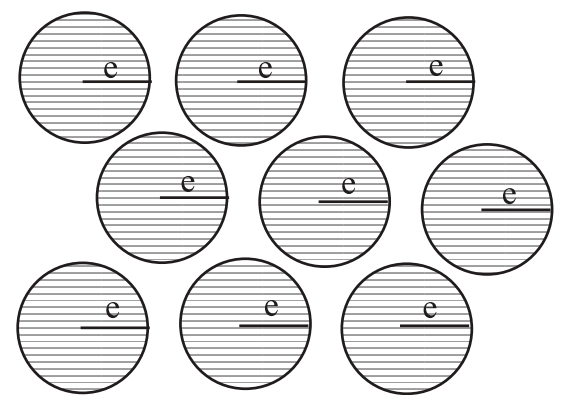
\includegraphics[scale=0.6]{../img/codewordsball.png}
\caption{Bola codeword yang tidak saling overlap}
\label{fig:codewordsball}
\end{figure}

Notasi umum kode biner adalah $(n,M,d)_2$. Kita bisa asumsikan ada $M$ bola yang tidak saling bersinggungan atau berpotongan, dengan radius bola $e$ seperti pada Gambar \ref{fig:codewordsball}. Jarak antara satu bola dengan bola yang lain adalah minimal $d$, sehingga didapatkan \refeq{eq:de}.
\begin{equation} \label{eq:de}
d = 2e + 1
\end{equation}

Sebuah kode biner $(n,M,d)_2$ dapat dibangkitkan dari kombinasi linear dari setiap baris pada generator matrix $[n,m,d]_2$ dimana $2^m = M$. Generator matriks $G$ adalah matriks berukuran $n \times m$, dapat juga disebut basis dari sebuah kode biner \cite{VanLint2016}. Contoh kode biner $(6,8,3)_2$ pada Gambar \ref{fig:binarycode683} dapat dibangkitkan dari generator matriks $[6,3,3]_2$ pada Gambar \ref{fig:generator633}. Asumsikan bahwa setiap baris dari $[6,3,3]_2$ adalah $g_1$, $g_2$, and $g_3$, lalu kode biner $(6,8,3)_2$ adalah semua kombinasi linear penjumlahan dari semua vektor dalam bentuk ${\lambda}_1 g_1 + {\lambda}_2 g_2 + {\lambda}_3 g_3$ dimana $\lambda{_i} \in \mathbb{F}_2^6$.

\begin{figure}
\centering
\begin{BVerbatim}
100110
010101
001011
\end{BVerbatim}
\caption{Generator matrix $[6,3,3]_2$}
\label{fig:generator633}
\end{figure}

\begin{figure}
\centering
\begin{BVerbatim}
1001101
0101011
0010111
\end{BVerbatim}
\caption{Generator matrix $[7,3,4]_2$}
\label{fig:generator734}
\end{figure}

\begin{figure}
\centering
\begin{BVerbatim}
0000000  1000111
0011101  1000111
0101011  1000111
0110110  1000111
\end{BVerbatim}
\caption{Perfect binary code $(7,8,4)_2$}
\label{fig:binarycode784}
\end{figure}

Dari sebuah kode biner, kita dapat membuat kode biner yang baru dengan memodifikasi kode biner yang sudah ada \cite{Huffman}. Modifikasi yang dapat dilakukan adalah menambah dan mengurangi kode. Dari sebuah kode biner $(n,M,d)_2$, dapat dilakukan pemotongan pada kolom tertentu sehingga kode biner menjadi $(n-1,M,d')_2$ dimana $d'=d \lor d'=d-1$. Begitu pula dengan penambahan kode, dari sebuah kode biner $(n,M,d)_2$, dapat dilakukan penambahan kode sehingga kode biner menjadi $(n+1,M,d')_2$ dimana $d'=d \lor d'=d+1$. 
 \cleardoublepage
    \chapter{METODE PENELITIAN}

Bab ini memaparkan tentang metodologi penelitian yang digunakan pada penelitian ini yaitu tahap analisis penyelesaian masalah dan implementasi.


\section{Desain dan analisis penyelesaian masalah}

Pada permasalahan pencarian Ulam non interaktif, penjawab tidak diperbolehkan menjawab sebelum penanya selesai menanyakan seluruh query. Ada dua pendekatan berbeda yang dapat dilakukan untuk menyelesaikan masalah tersebut, yaitu menggunakan repetisi pencarian biner dan menggunakan kode biner. Perlu diketahui bahwa kedua solusi tersebut tidak saling berhubungan.


\subsection{Solusi menggunakan kode biner}

Kita tahu bahwa permasalahan Ulam dengan ruang pencarian $M$ dan maksimal bohong $e$ dapat deselesaikan dengan membuat $q$ query yang jika ditranspose akan membentuk kode biner $(n,M,d)_2$ dimana $d = 2*e+1$. Oleh karena itu tahap selanjutnya adalah jika diketahui $M$ dan $d$, bagaimana membuat seminimal mungkin $n$ agar kode biner $(n,M,d)_2$ valid. Langkah utama untuk membuat kode biner tersebut dengan $M$ dan $e$ yang diketahui adalah dengan menambahkan kode secara iteratif agar minimal jarak Hamming kode biner mencapai $e$.

Gambar \ref{fig:hamming1} menunjukkan ilustrasi jika $M = 8$, $n = 3$, dan $d = 1$. Tabel pada gambar  menunjukkan jarak Hamming antar codeword $x$ dan $y$, sehingga dapat disimpulkan jarak Hamming minimal adalah 1. Gambar \ref{fig:hamming2} adalah penambahan dua kode dari Gambar \ref{fig:hamming1} sehingga $n = 5$ dan $d = 2$.

\begin{figure}
\centering
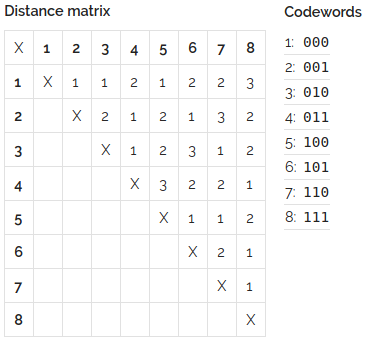
\includegraphics[scale=0.7]{../img/hamming1.png}
\caption{Hasil tabel jarak Hamming pada $(3,8,1)_2$}
\label{fig:hamming1}
\end{figure}

Diagram alir algoritma untuk menyelesaikan permasalahan Ulam non interaktif ada pada Gambar \ref{fig:flow_binarycode}. Setelah dilakukan input ruang pencarian $M$ dan maksimal bohong $e$, simpan $M$ untuk digunakan pada saat output query terakhir. Ubah $M$ menjadi perpangkatan dua terdekat, karena algoritma selanjutnya hanya dapat berjalan jika $M$ adalah perpangkatan dua. Pada subbab selanjutnya akan dijelaskan algoritma untuk menggunakan query generator dan juga algoritma utama untuk menyelesaikan permasalahan Ulam non interaktif.

\begin{figure}
\centering
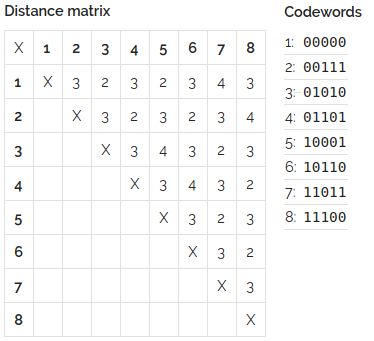
\includegraphics[scale=0.7]{../img/hamming2.png}
\caption{Hasil tabel jarak Hamming pada $(5,8,2)_2$}
\label{fig:hamming2}
\end{figure}

Proses pencarian mendalam (\textit{exhaustive search}) menggunakan pendekatan \textit{greedy} akan dilakukan sebagai pra proses dan hasil pra proses tersebut akan langsung dimasukkan ke dalam kode sumber solusi, karena proses pencarian mendalam memiliki kompleksitas $O(M^3)$ sedangkan jika dilakukan sebagai pra proses dan dimasukkan langsung ke dalam kode sumber solusi sebagai array akan mengurangi kompleksitas menjadi $O(1)$. Namun untuk keperluan pengujian, algoritma kode biner tanpa tabel pencarian (algoritma kode biner yang melakukan proses pencarian mendalam) akan dibandingkan dengan algoritma kode biner dengan tabel pencarian (proses pencarian mendalam dilakukan sebagai pra proses).

\begin{figure}
\centering
\begin{tikzpicture}[node distance=2cm,on grid,auto]
% nodes
\node (n0) [start] {Start};
\node (n1) [io,below of=n0] {Input $M$, $e$};
\node (n2) [process,below of=n1,align=center] {$real\_M = M$\\$m$ = ceil($\log_2(M)$)\\$M=2^m$};
\node (n3) [process,below of=n2,align=center] {$code$ = Generate all possible query using query generator};
\node (n4) [process,below of=n3,align=center] {$code\_order$ = Preloaded exhaustive search($2 \leq 2^m  \leq 4096$, 16)};
\node (n5) [process,below of=n4] {$minimal$ = Generate minimal query};
\node (n6) [process,below of=n5] {$queries$ = Generate actual query};
\node (n7) [io,below of=n6] {Print all the $queries$};
\node (n8) [start,below of=n7] {End};
% arrows
\draw[arrow] (n0) -- (n1);
\draw[arrow] (n1) -- (n2);
\draw[arrow] (n2) -- (n3);
\draw[arrow] (n3) -- (n4);
\draw[arrow] (n4) -- (n5);
\draw[arrow] (n5) -- (n6);
\draw[arrow] (n6) -- (n7);
\draw[arrow] (n7) -- (n8);
\end{tikzpicture}
\caption{Diagram alir solusi menggunakan pembobotan Berlekamp}
\label{fig:flow_binarycode}
\end{figure}


\subsubsection{Algoritma pembangkitan query}

Untuk membuat kode biner $(n,M,d)_2$, maka diperlukan algoritma untuk membangkitkan kode. Karena setiap satu query adalah hasil transpose dari sebuah kolom pada kode biner, setiap kolom pada kode biner dapat dibuat dari bitstring pembangkit $s = \mathbb{F}_2^m$ yang jika diubah menjadi integer akan memiliki rentang $0 \leq s < M$. Oleh karena itu ada $M-1$ macam $s$ karena $s=0$ akan menghasilkan query $\vec{0}$ yang tidak akan menghasilkan jarak Hamming pada kode biner.

Algoritma untuk membuat sebuah query dengan code generator ditunjukkan pada Kode Sumber \ref{alg:generate_query}. Input dari fungsi ini adalah ruang pencarian $M$ dan bilangan bulat $s$ yang akan diubah menjadi sebuah query. Pertama-tama siapkan bilangan bulat $0 \leq i < M$ untuk perulangan kombinasi linier pada $s$ seperti yang ditunjukkan pada baris \ref{alg:kombinasi_linier_for}. Lalu kalikan semua bit dari $s$ dan $i$ seperti yang ditunjukkan pada baris \ref{alg:kombinasi_linier}. Lalu jumlahkan semua bit hasil perkalian $s \cdot i$ seperti yang ditunjukkan pada baris \ref{alg:counting_bit_set}. Lalu hasil semua kombinasi linear akan ditampung pada string $query$ seperti yang ditunjukkan pada baris \ref{alg:save_query}. Total query akan memiliki panjang $M$.

\begin{algorithm}[h]
\caption{Algoritma membuat sebuah query dengan code generator}
\label{alg:generate_query}
\Fn{generate\_query($M$, $s$)}{
\KwData{$M$ search space, $s$ initial generator number}
\KwResult{$query$}
  $query$ = ""\;
  \For{$i = 0$ \KwTo $M$}{\label{alg:kombinasi_linier_for}
    $bitstring = i\ \&\ s$\;\label{alg:kombinasi_linier}
    $binary = 0$\;
    \While{$bitstring$}{\label{alg:counting_bit_set}
      $binary \mathrel{\wedge}= bitstring\ \&\ 1$\;
      $bitstring \mathrel{>>}= 1$\;
    }
    $query \mathrel{+}= binary$\;\label{alg:save_query}
  }
  \Return $query$\;
}
\end{algorithm}

\begin{figure}
\centering
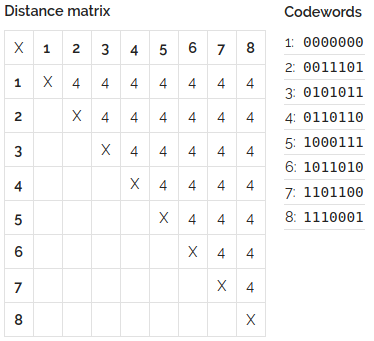
\includegraphics[scale=0.5]{../img/hamming3.png}
\caption{Hasil tabel jarak Hamming pada $M=8$ dan $n=7$}
\label{fig:perfect8}
\end{figure}

\begin{figure}
\centering
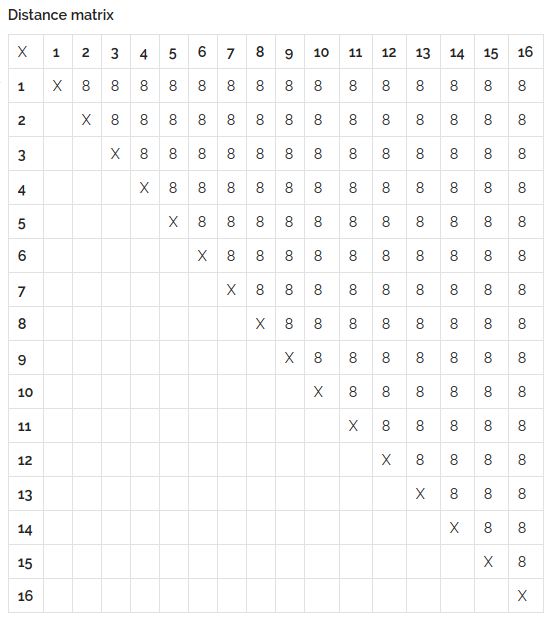
\includegraphics[scale=0.45]{../img/perfect16.png}
\caption{Hasil tabel jarak Hamming pada $M=16$ dan $n=15$}
\label{fig:perfect16}
\end{figure}

Setelah melakukan percobaan menggunakan seluruh $M-1$ query untuk $M$ ruang pencarian, didapatkan seluruh jarak hamming setiap codeword adalah $M/2$. Gambar \ref{fig:perfect8} adalah contoh pada $M=8$ dan $n=7$. Lalu Gambar \ref{fig:perfect16} adalah contoh pada $M=16$ dan $n=15$. Dari hasil tersebut dapat disimpulkan bahwa dengan melakukan seluruh $M-1$ macam query dengan generator untuk ruang pencarian $M$, akan didapatkan kode biner dengan $d=M/2$. Kode biner pada Persamaan \ref{eq:perfectbinarycode} disebut sempurna karena seluruh jarak Hamming pada setiap codeword yang berbeda bernilai $d = M/2$.

\begin{equation}
\label{eq:perfectbinarycode}
\text{Terdapat kode biner sempurna }(M-1, M, M/2)_2
\end{equation}

\begin{align}
q_{rep} &= d\ \backslash\ (M/2) \label{eq:qrep} \\
d_{mod} &= d \text{ mod } (M/2) \label{eq:dmod}
\end{align}

Oleh karena itu jika kita membutuhkan query yang menghasilkan $d = M/2$, maka gunakan seluruh $M-1$ query dengan generator. Sedangkan jika kita membutuhkan query yang menghasilkan $d < M/2$, pilih sesedikit mungkin $n$ query agar menghasilkan $d$ yang dibutuhkan. Dari kebutuhan tersebut, dibuatlah rumus $q_{rep}$ dan $d_{mod}$. Nilai $q_{rep}$ yang didapat dari Persamaan \ref{eq:qrep} adalah jumlah perulangan yang dilakukan terhadap $M-1$ query untuk mencapai solusi. Nilai $d_{mod}$ yang didapat dari Persamaan \ref{eq:dmod} adalah sisa jarak Hamming $d$ yang dibutuhkan untuk mencapai solusi. Cara untuk mencari jumlah query sisa untuk menghasilkan jarak Hamming distance $d_{mod}$ ada pada subbab selanjutnya.


\subsubsection{Pencarian mendalam dengan greedy}

Algoritma solusi menggunakan generator matrix harus membuat urutan $s$ tertentu sedemikian hingga seminimal mungkin jumlah query $n$ yang dihasilkan dari $\vec{s} = \{s_1, \ldots, s_n\}$ akan menghasilkan semaksimal mungkin jarak Hamming $d$. Untuk itu dibuatlah algoritma pencarian mendalam \textit{exhaustive search} dengan pendekatan \textit{greedy} untuk mendapatkan urutan $\vec{s}$ yang paling optimal seperti yang ditunjukkan pada Kode Sumber \ref{alg:exhaustive_search}.

Pertama-tama program membuat seluruh $M-1$ kemungkinan query menggunakan algoritma pembangkit query sehingga terbentuk $M-1$ query seperti yang ditunjukkan pada baris \ref{alg:pre_binary_code}. Lalu pada baris \ref{alg:best_order_loop}, program melakukan perulangan pencarian mendalam untuk membuat query sampai batas jarak Hamming $d$ yang diinginkan menggunakan. Dilakukan pendekatan \textit{greedy} karena \textit{global optimum} yang dicari adalah sebesar mungkin nilai jarak minimal dengan query sesedikit mungkin. \textit{Global optimum} tersebut dapat didapat dengan mencari \textit{local optimum} di setiap iterasi.

Pada algoritma \textit{greedy}, fungsi seleksi untuk memilih kandidat query terbaik pada setiap iterasi ada empat macam:
\begin{enumerate}
  \item Jarak minimum terbesar;
  \item Jarak minimum terbesar lalu jarak maximum terkecil;
  \item Pengurangan jarak maximum dengan jarak minimum terkecil;
  \item Jarak minimum terbesar lalu jumlah angka yang memiliki nilai minimum terkecil.
\end{enumerate}

Keempat fungsi seleksi tersebut ditentukan karena \textit{global optimum} yang dicari adalah jarak minimum terbesar, selisih nilai jarak maximum dan jarak minimum harus sekecil mungkin, dan query yang dihasilkan dapat menghabiskan sebanyak mungkin angka dengan jarak minimum. Keempat fungsi seleksi  akan diuji untuk dipilih fungsi seleksi terbaik dan digunakan pada program utama.

Pada baris \ref{alg:best_search_loop}, program melakukan perulangan untuk mencoba semua macam query yang belum digunakan untuk mencari yang terbaik, dan mengabaikan query yang sudah digunakan pada baris \ref{alg:skip_used_code}. Untuk mencari query yang terbaik pada state \texttt{order\_pointer}, parameter yang digunakan adalah sesuai dengan empat fungsi seleksi yang ditunjukkan pada baris \ref{alg:greedy_selection}. Setelah setiap satu pencarian best query pada satu state, program akan memperbarui jarak Hamming seperti yang ditunjukkan pada baris \ref{alg:update_distance}, lalu masukkan kandidat query terbaik ke \texttt{code\_order} seperti yang ditunkukkan pada baris \ref{alg:update_order}.

\begin{algorithm}[h]
\caption{Algoritma mencari urutan bibit generator terbaik}
\label{alg:exhaustive_search}
\Fn{exhaustive\_search($M$, $e$)}{
\KwData{$M$ search space, $e$ max lies allowed}
\KwResult{$code\_order$}
  $code[M] = [\ ]$\;\label{alg:var_code}
  $code\_distance[M] = [\ ]$\;\label{alg:var_code_distance}
  $code\_min=0$\;\label{alg:var_code_min}
  $code\_order[M] = [\ ]$\;\label{alg:var_code_order}
  
  \For{$i = 1$ \KwTo $M$}{\label{alg:pre_binary_code}
    $code[i]$ = generate\_query($M$, $i$)\;
  }

  \While{$code\_min < d$}{\label{alg:best_order_loop}
    $most\_min = 0$\;\label{alg:most_minimal_distance}
    $least\_min\_count = \infty$\;\label{alg:least_minimal_member}
    % /* each loop find the one best code order candidate */
    \For{$i = 1$ \KwTo $M$}{\label{alg:best_search_loop}
      \lIf{$code[i]$ already used}{continue}\label{alg:skip_used_code}
      $min$ = minimal hamming distance if using $code[i]$\;\label{alg:test_distance}
      $min\_count$ = how many node which have hamming distance is $min$\;\label{alg:minmax}
      \If{\text{meet the greedy selection function}}{\label{alg:greedy_selection}
        $best = i$\;
        $most\_min = min$\;\label{alg:save_the_best}
        $least\_min\_count = min\_count$\;
      }
    }

    $code\_min = \infty$\;
    \For{$j = 1$ \KwTo $M$}{\label{alg:update_distance}
      $code\_distance[j] \mathrel{+}= (code[best][0] != code[best][j])$\;
      \If{$code\_distance[j] < code\_min$} {
        $code\_min = code\_distance[j]$\;
      }
    }

    $code\_order$[$order\_pointer$++] = $best$\;\label{alg:update_order}
  }
  \Return $code\_order$\;
}
\end{algorithm}

Keluaran dari algoritma ini dengan inputan $2 \leq 2^m \leq 4096$ dan $e=16$ serta dengan fungsi seleksi terpilih akan menghasilkan sejumlah query beserta urutan seednya. Hasil query tersebut akan dimasukkan langsung ke dalam code pada solusi optimal pencarian Ulam non interaktif yang akan dijelaskan pada subbab selanjutnya.


\subsubsection{Algoritma mencari query minimal}

Dari keluaran algoritma mencari urutan kode biner, akan dibuat algoritma mencari query minimal untuk menghasilkan array $minimal$ berisi pasangan \textit{key-value}, minimal jarak Hamming $d$ sebagai \textit{key} dan $n$ jumlah query yang dibutuhkan untuk membuat codeword dengan jarak minimal jarak Hamming $d$. Pembuatan array $minimal$ pada baris \ref{alg:minimal}. Array $minimal$ akan digunakan untuk mendapatkan nilai $d_{mod}$ yang sebelumnya dijelaskan pada Persamaan \ref{eq:dmod}. Dari algoritma ini, kita bisa mendapatkan $q_{mod}$ dari $d_{mod}$ dengan memasukkan $d_{mod}$ ke index pada array $minimal$ seperti pada Persamaan \ref{eq:qmod}.

\begin{equation}
\label{eq:qmod}
q_{mod} = minimal[d_{mod}]
\end{equation}

\begin{algorithm}[h]
\caption{Algoritma mencari query minimal}
\label{alg:generate_minimal_query}
\KwResult{$minimal$ array}
  $minimal = [\ ]$\;
  $distances[M] = [\ ]$\;

  \For{$i = 0$ \KwTo $M-1$}{
  % for (int i = 0; i < M-1 \&\& min < d; ++i) {
    $min = \infty$\;
    % /* binary start from 0 to M */
    $query = \text{generate\_query}(M, code\_order[m][i])$\;
    update the $distances$ after $query$\;
    $min$ = min($distances$)\;
    $minimal[min] = i$\;\label{alg:minimal}
    \lIf{$min \geq d$}{break}
  }
  \Return $minimal$\;
\end{algorithm}


\subsubsection{Menyatukan query repetisi dan query mod}

Setelah mendapatkan array $minimal$, tahap terakhir adalah menyatukan query. Total query yang dihasilkan ada pada Persamaan \ref{eq:total_query}. Query tersebut terdiri dari $q_{rep} \times M/2$ seperti ditunjukkan pada baris \ref{alg:qrep} dan $q_{mod}$ seperti ditunjukkan pada baris \ref{alg:dmod}.

\begin{equation}
\label{eq:total_query}
q = q_{rep} \times (M-1) + q_{mod}
\end{equation}

\begin{algorithm}[h]
\caption{Algoritma membuat query yang sebenarnya}
\label{alg:actual_query}
\KwResult{$solutions$}
  $qrep$ = $d/(M/2)$\;
  $dmod$ = $d$ mod $(M/2)$\;
  $solution = [\ ]$\;

  \For{$i = 0$ \KwTo $qrep$}{ \label{alg:qrep}
    \For{$j = 0$ \KwTo $M-1$}{
      $solution$.push($code[j]$.substr($real\_M$))\;
    }
  }
  \For{$i = 0$ \KwTo $minimal[dmod]$}{ \label{alg:dmod}
    $solution$.push($code[code\_order[i]]$.substr($real\_M$))\;
  }

  \Return $solution$\;
\end{algorithm}

\subsection{Solusi menggunakan repetisi pencarian biner}

Algoritma pencarian biner ada pada Kode Sumber \ref{alg:repetisi_biner}. Baris \ref{alg:for_qb} menunjukkan perulangan untuk setiap jenis query $q_b$. Nilai $q_b$ adalah hasil $\log_2$ dari M, lalu dibulatkan ke atas karena $M$ harus merupakan perpangkatan dari 2 sehingga nilai $q_b = \text{ceil}(\log_2(M))$. Baris \ref{alg:for_m} menunjukkan perulangan untuk membuat setiap satu jenis query pencarian biner. Baris \ref{alg:find_bit} menunjukkan proses untuk mencari bit pada posisi tertentu pada sebuah integer \cite{bithack}. Setiap query akan diulang sebanyak $qe$ seperti yang ditunjukkan pada baris \ref{alg:for_qe}.

\begin{algorithm}[h]
\caption{Algoritma repetisi pencarian biner}
\label{alg:repetisi_biner}
\Fn{repetitive\_binary\_search($M$, $e$)}{
\KwData{$M$ search space, $e$ max lies allowed}
\KwResult{$queries$}
  $queries = [\ ]$\;
  $qb = \text{ceil}(\log_2(M))$\;
  $qe = 2*e + 1$\;
  $twopower = 1$\;
  \For{$i = 0$ \KwTo $qb$}{\label{alg:for_qb}
    $string = ""$\;
    \For{$j = 0$ \KwTo $M$}{\label{alg:for_m}
      \leIf{$j\ \&\ twopower$}{\label{alg:find_bit}
        $string \mathrel{+}= "1"$\;
      }{
        $string \mathrel{+}= "0"$\;
      }
    }
    \For{$j = 0$ \KwTo $qe$}{\label{alg:for_qe}
      $queries$.push($string$)\;
    }
    $twopower \mathrel{*}= 2$\;
  }
  \Return $queries$\;
}
\end{algorithm}


\section{Desain pengujian keabsahan algoritma}

Untuk menguji kebenaran query akan dibuat program yang dapat menguji query yang dihasilkan oleh algoritma solusi, agar tidak ada satu set pun yang menyebabkan ada lebih dari satu kemungkinan nilai $x$. Isi dari program pengujian kebenaran algoritma adalah mengecek apakah minimal jarak Hamming setiap query yang berbeda pada setiap kasus uji bernilai minimal $2e+1$ seperti yang ditunjukkan pada Kode Sumber \ref{alg:query_assert}. Variabel $dist$ pada baris \ref{alg:assert_distvar} digunakan untuk menyimpan jarak antara bit ke-0 dengan seluruh bit yang lain. Baris \ref{alg:assert_dist} menunjukkan bahwa jarak akan bertambah setiap ada perbedaan nilai bit.

\begin{algorithm}[h]
\caption{Algoritma pengujian kebenaran query}
\label{alg:query_assert}
\Fn{query\_checker\_search($M$, $e$, $queries$)}{
\KwData{$M$ search space, $e$ max lies allowed, $queries$ to be checked}
\KwResult{$is\_win$}
  $dist[M] = [0, \ldots, 0]$\;\label{alg:assert_distvar}
  \For{$i = 1$ \KwTo $queries$.size}{
    $dist[j] \mathrel{+}= (queries[i][0] \mathrel{!}= queries[i][j])$\;\label{alg:assert_dist}
  }
  \For{$i = 1$ \KwTo $queries$.size} {
    \If{$dist[i] < 2*e+1$} {
      \Return false\;
    }
  }
  \Return true\;
}
\end{algorithm}


\section{Implementasi algoritma}

Implementasi merupakan tahap untuk membangun algoritma yang akan digunakan. Pada tahap ini dilakukan implementasi dari rancangan struktur data yang akan dimodelkan sesuai dengan permasalahan. Implementasi dilakukan dengan menggunakan bahasa pemrograman C++ agar dapat disubmit ke SPOJ. Selain itu akan dilakukan implementasi program dalam bahasa C++ yang dapat mengecek kebenaran query dengan menghitung apakah jarak Hamming dari query sudah melampaui $2e+1$.

% Implementasi dalam bahasa coffeescript untuk menghasilkan halaman web. Visualisasi dalam bentuk web digunakan untuk mencari pola pada query karena penampilan yang lebih dapat dipahami. Selain itu akan dibuat visualisasi untuk memudahkan pembacaan jarak Hamming pada kode biner. Aplikasi web akan menerima input, lalu menampilkan visualisasi sesuai dengan kebutuhan.
 \cleardoublepage
    \chapter{HASIL DAN PEMBAHASAN}

Bab ini memaparkan tentang hasil dan pembahasan pada metode-metode yang digunakan pada penelitian ini.

\section{Lingkungan Uji Coba}

Uji coba dilakukan pada perangkat dengan spesifikasi berikut.

\begin{enumerate}
  \item Perangkat Keras
  \begin{enumerate}
    \item Processor Intel® Core™ i7-7400 CPU @ 3.00GHz (4 CPUs), ~3.0GHz
    \item Random Access Memory 8192MB
  \end{enumerate}
  \item Perangkat Lunak
  \begin{enumerate}
    \item Sistem Operasi Linux Ubuntu 16.04
    \item Bahasa Pemrograman C++
    \item gcc 5.4.0
  \end{enumerate}
\end{enumerate}


\section{Penyelesaian menggunakan repetisi pencarian biner}

Algoritma repetisi pencarian biner menghasilkan maksimal sebanyak $\log_2(M) \cdot (2e + 1)$ query non interaktif pada setiap kasus uji. Algoritma pencarian biner ada pada Kode Sumber \ref{alg:repetisi_biner}. Baris \ref{alg:for_qb} menunjukkan perulangan untuk setiap jenis query $qb$. Nilai $qb$ adalah hasil $\log_2$ dari M, lalu dibulatkan ke atas karena $M$ harus merupakan perpangkatan dari 2 sehingga nilai $qb = \text{ceil}(\log_2(M))$. Baris \ref{alg:for_m} menunjukkan perulangan untuk membuat setiap satu jenis query pencarian biner. Baris \ref{alg:find_bit} menunjukkan proses untuk mencari bit pada posisi tertentu pada sebuah integer \cite{bithack}. Setiap query akan diulang sebanyak $qe$ seperti yang ditunjukkan pada baris \ref{alg:for_qe}.

\begin{algorithm}[h]
\caption{Algoritma repetisi pencarian biner}
\label{alg:repetisi_biner}
\Fn{repetitive\_binary\_search($M$, $e$)}{
\KwData{$M$ search space, $e$ max lies allowed}
\KwResult{$queries$}
  $queries = [\ ]$\;
  $qb = \text{ceil}(\log_2(M))$\;
  $qe = 2*e + 1$\;
  $twopower = 1$\;
  \For{$i = 0$ \KwTo $qb$}{\label{alg:for_qb}
    $string = ""$\;
    \For{$j = 0$ \KwTo $M$}{\label{alg:for_m}
      \eIf{$j\ \&\ twopower$}{\label{alg:find_bit}
        $string \mathrel{+}= "1"$\;
      }{
        $string \mathrel{+}= "0"$\;
      }
    }
    \For{$j = 0$ \KwTo $qe$}{\label{alg:for_qe}
      $queries$.push($string$)\;
    }
    $twopower \mathrel{*}= 2$\;
  }
  \Return $queries$\;
}
\end{algorithm}

\subsection{Skenario Uji Coba}

Subbab ini akan menjelaskan hasil pengujian program penyelesaian permasalahan. Algoritma disubmit ke SPOJ dalam bahasa C, menghasilkan penilaian yang ditunjukkan pada Tabel \ref{tab:score_repetitive}. Karena ini adalah algoritma yang pasti benar dengan cara termudah, maka dapat diasumsikan bahwa skor yang didapat dari algoritma ini adalah skor minimal yang dapat menjadi tolok ukur keberhasilan algoritma yang lain.

\begin{table}[h!]
\caption{Hasil algoritma repetisi pencarian biner pada SPOJ}
\label{tab:score_repetitive}
\begin{center}
\begin{tabular} {|l|l|}
\hline
ID & 20152331 \\ \hline
Tanggal & 2017-09-14 06:08:19 \\ \hline
Skor & 42,787,090 \\ \hline
Waktu & 0.00 \\ \hline
Memori & 2.7M \\ \hline
\end{tabular}
\end{center}
\end{table}

\section{Penyelesaian menggunakan kode biner}
 \cleardoublepage
    \chapter{KESIMPULAN}

Bab ini membahas mengenai kesimpulan yang dapat diambil dari hasil uji coba yang telah dilakukan sebagai jawaban dari rumusan masalah yang dikemukakan. Selain kesimpulan, juga terdapat saran yang ditujukan untuk pembangunan penelitian lebih lanjut.

\section{Kesimpulan}

\section{Saran} \cleardoublepage
    % \chapter{KESIMPULAN}

Berdasarkan penjabaran di bab-bab sebelumnya, dapat disimpulkan beberapa poin terkait penyelesaian permasalahan permainan Ulam non interaktif.

 \cleardoublepage

  \backmatter
    \printbibliography
    \chapter{BIODATA PENULIS}

\begin{wrapfigure}{l}{0.3\textwidth}
  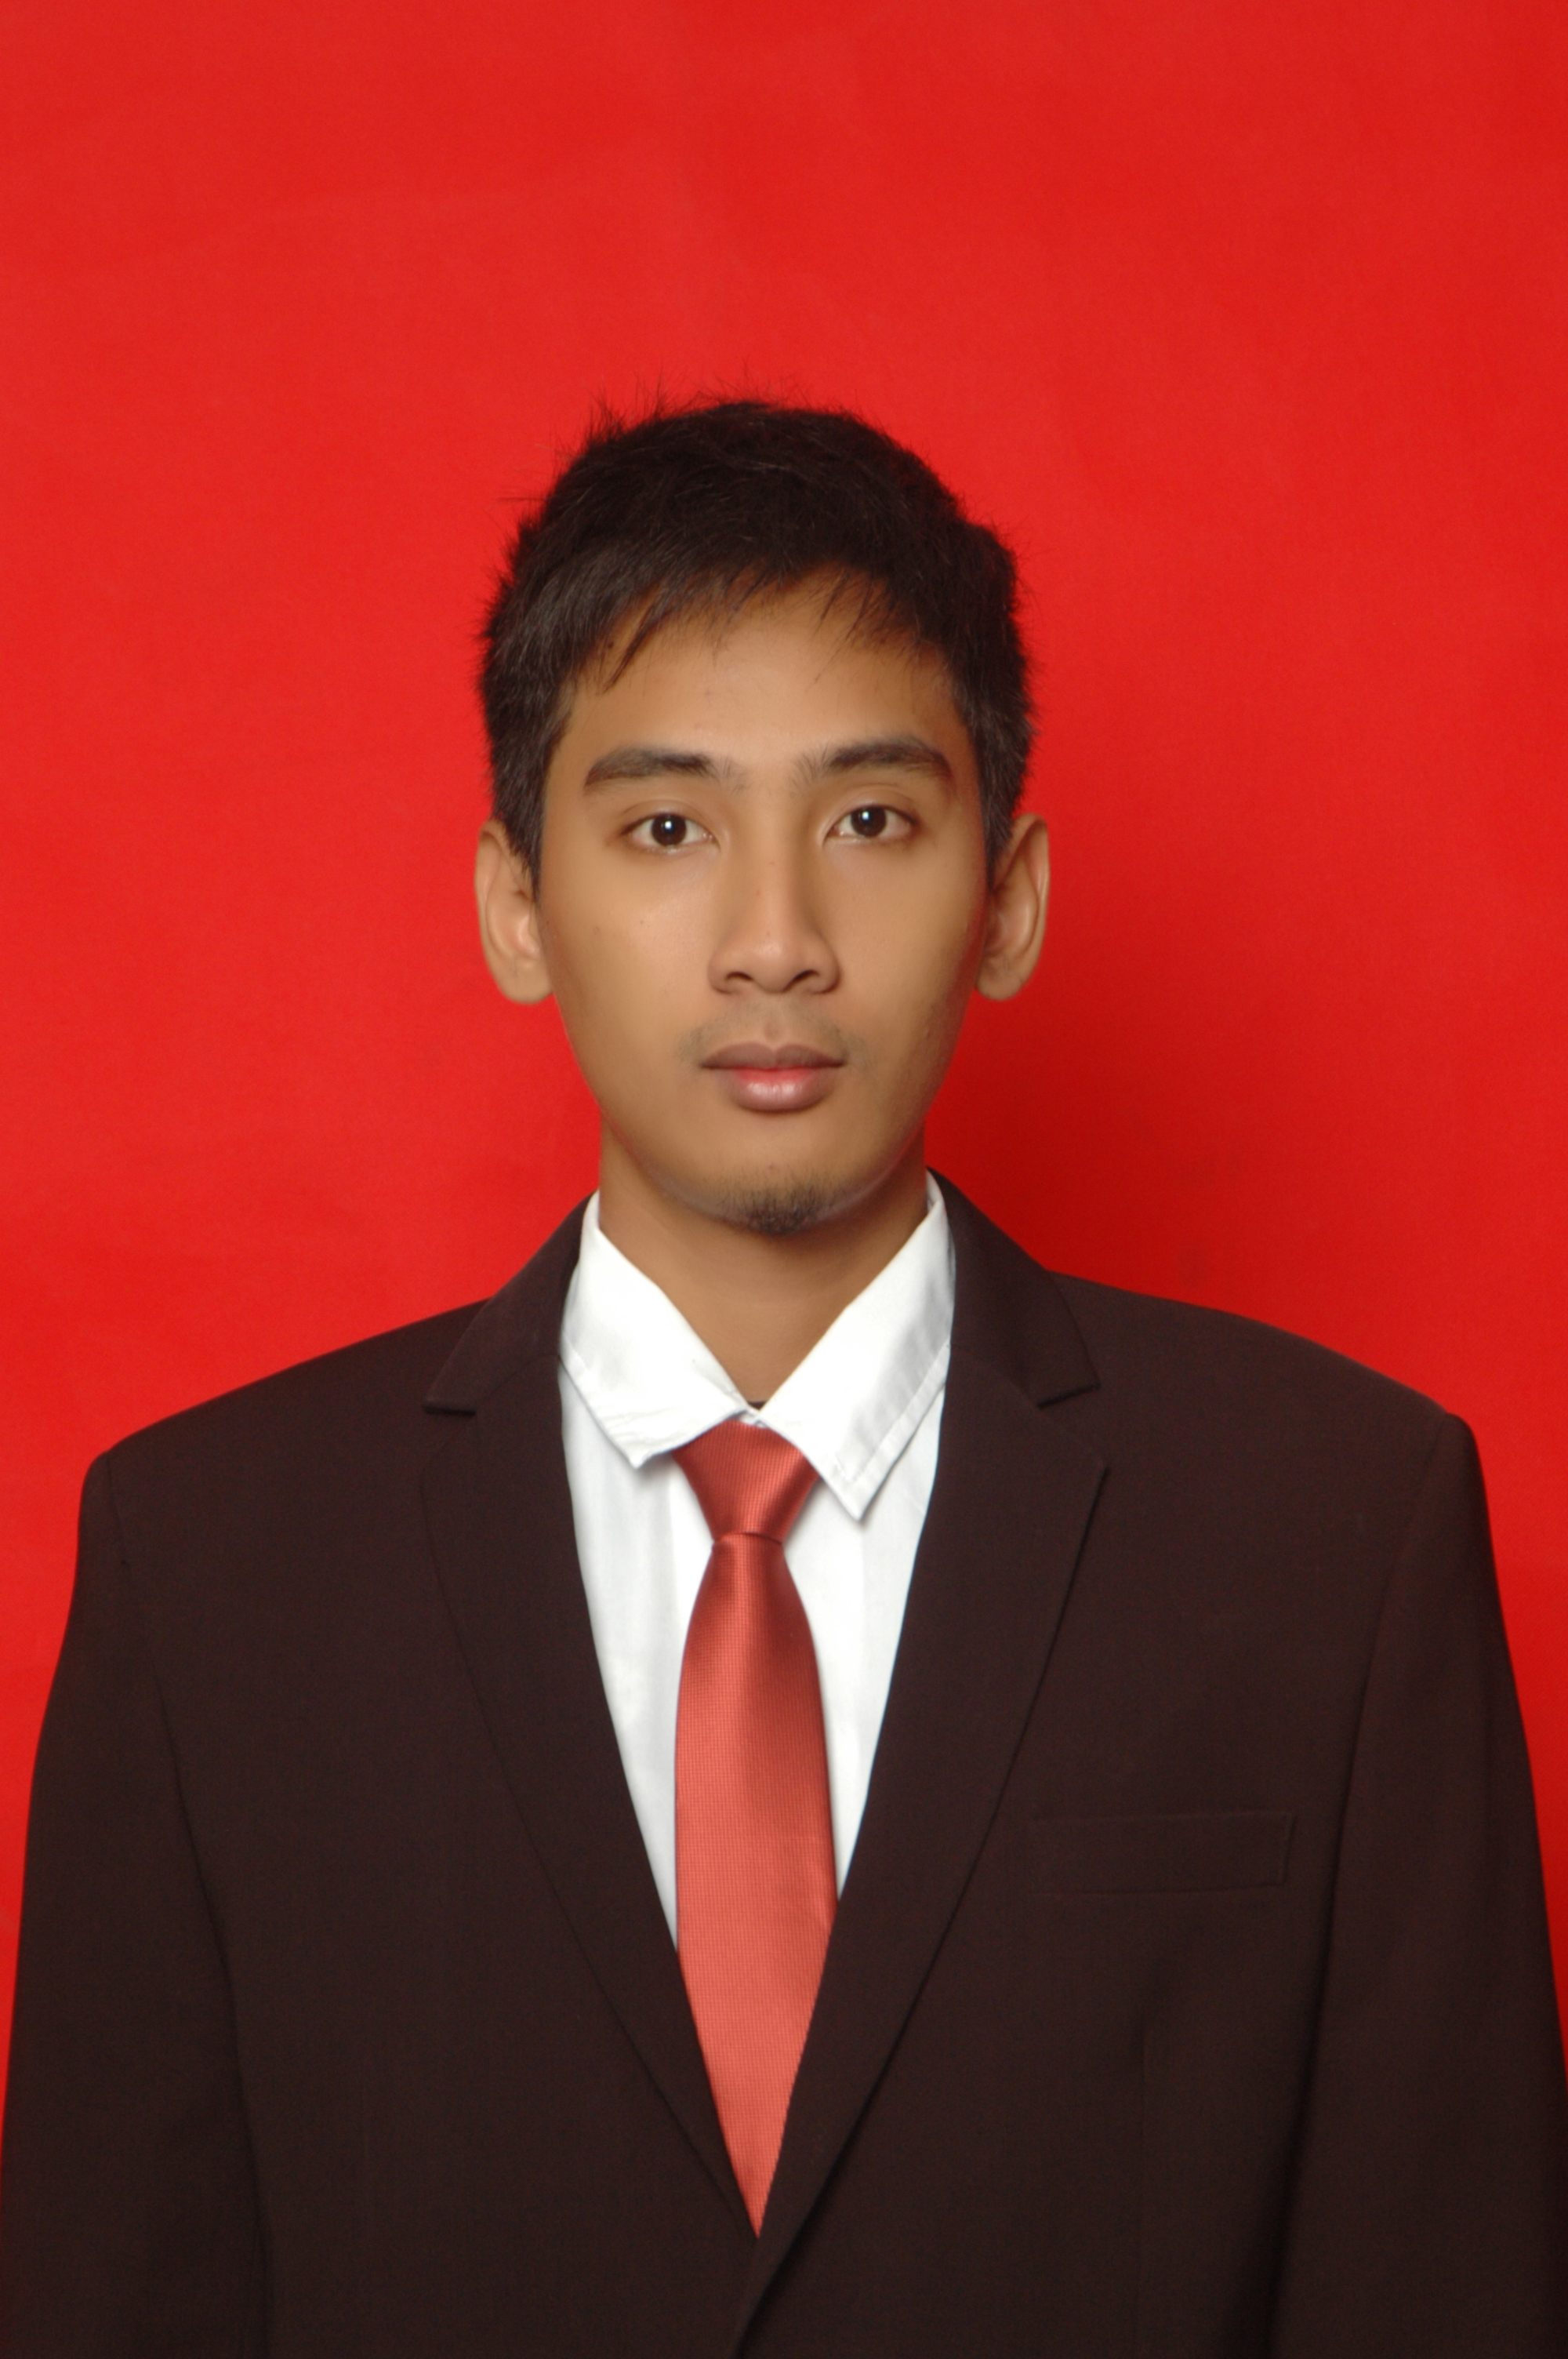
\includegraphics[height=0.3\textheight]{../img/foto.jpg}
\end{wrapfigure}

Penulis, Risyanggi Azmi Faizin, lahir di kota Surabaya pada tanggal 29 Juli 1993. Penulis dibesarkan di kota Sidoarjo, Jawa Timur. 

Penulis menempuh pendidikan formal di SD Al-Hikmah Surabaya (1999-2005), SMP Al-Hikmah Surabaya (2005-2008), SMAN 15 Surabaya (2008-2011). Pada tahun 2012, penulis melanjutkan pendidikan S1 \jurusanbaru\ \fakultasbaru\ di Institut Teknologi Sepuluh Nopember, Surabaya, Jawa Timur.

Di \jurusanbaru, penulis mengambil bidang minat Algoritma dan Pemrograman atau biasa disingkat menjadi Alpro dan memiliki ketertarikan di bidang desain web, perancangan perangkat lunak, big data, dan Pemodelan 3D. Penulis aktif sebagai vokalis di Paduan Suara Mahasiswa ITS. Penulis dapat dihubungi melalui alamat surel (email) risyanggi@gmail.com.

\end{document}